\head{Ноябрь}{Ознакомительная самостоятельная работа по теме «Графы».}

\begin{thm}
    В кружке танцев каждая девочка познакомилась с 6 мальчиками и 7 девочками, а каждый мальчик -- с 3 девочками и 4 мальчиками. Кого в кружке больше: мальчиков или девочек?
\end{thm}

\begin{thm}
    Какие рисунки задают один и тот же граф? 
\end{thm}

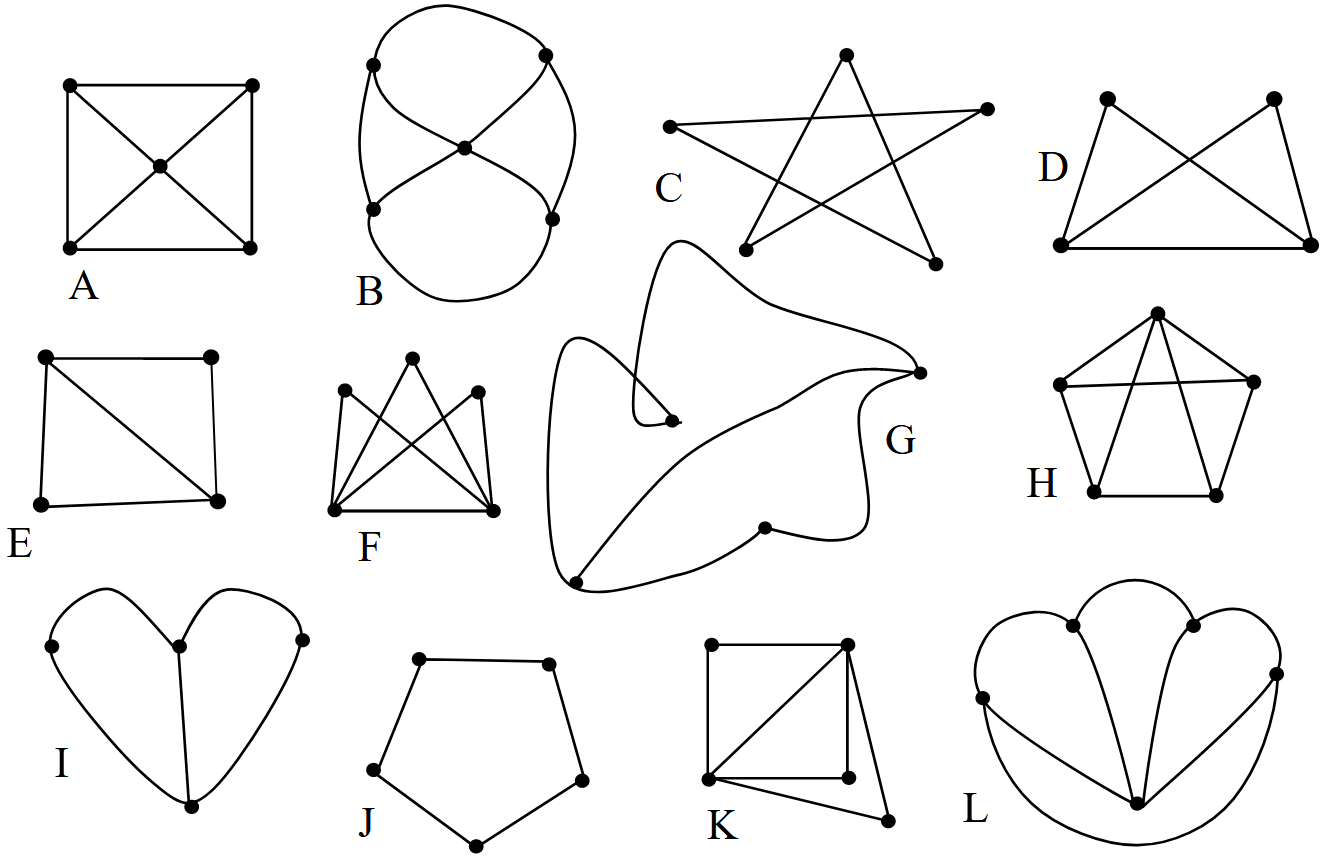
\includegraphics[width=0.95\columnwidth]{img/10.0.0 img1.png}

\begin{figure}[H]
\begin{minipage}{0.7\linewidth}
    \begin{thm}
        Докажите, что в любом графе с числом вершин не менее двух найдутся две вершины одинаковой степени.
    \end{thm}
\end{minipage}
    \hfill
\begin{minipage}{0.29\linewidth}
    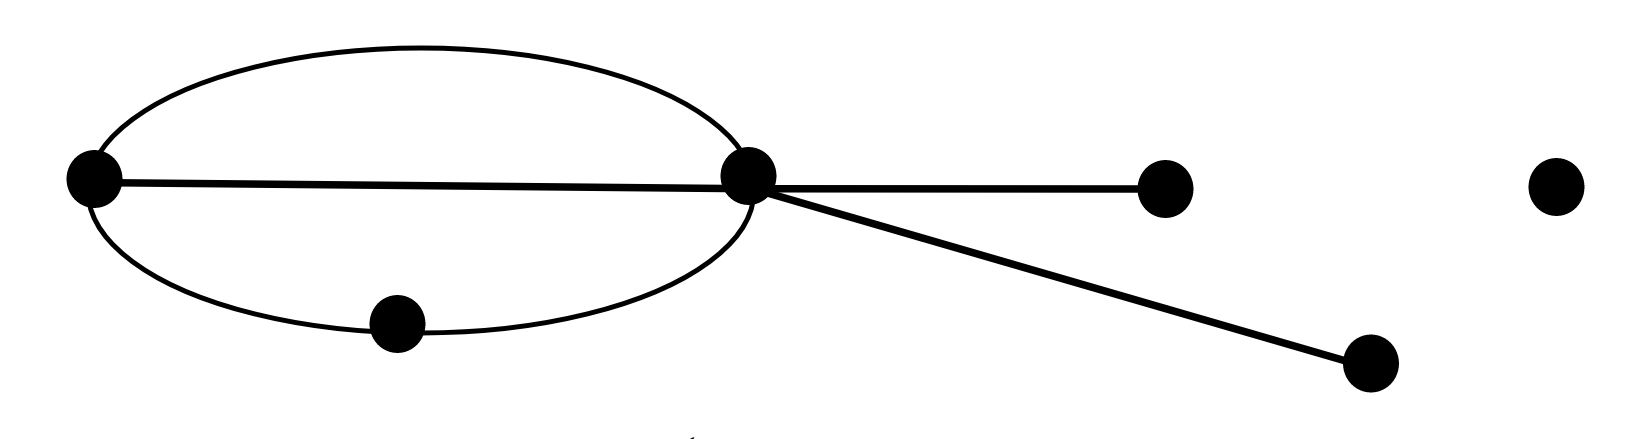
\includegraphics[width=0.95\columnwidth]{img/10.0.0 img2.png}
\end{minipage}
\end{figure}

\begin{thm}
    Запиши степени всех вершин графов $B$.
\end{thm}

\begin{thm}
    Проходит волейбольный турнир школы по круговой системе (каждая команда играет с каждой ровно один раз). Участвует 17 команд. В том числе и команда 8 класса. В некоторый момент времени оказалось, что все команды (кроме команды 8) сыграли разное количество матчей. Сколько матчей к этому моменту сыграла команда 8 класса?
\end{thm}

\begin{thm}
    В стране Миллениум некоторые города связаны между собой авиалиниями. Из столицы выходит 2013 авиалиний, из города Тьма--Таракань -- одна, а из всех остальных городов -- ровно по 2012 авиалинии. Можно ли из Тьмы--Таракани добраться в столицу?
\end{thm}

\begin{thm}
    В графе $n$ вершин. Степень каждой из них не меньше $\dfrac{n - 1}{2}$. Докажите, что граф связен.
\end{thm}

\begin{thm}
    В однокруговом турнире по настольному теннису каждый участник одержал четыре победы. Сколько человек участвовало в турнире?
\end{thm}

\begin{thm}
    Дайте определение эйлерова графа.
\end{thm}